\section{Figures}\label{sec:figures}

\begin{figure}[t]
\centering
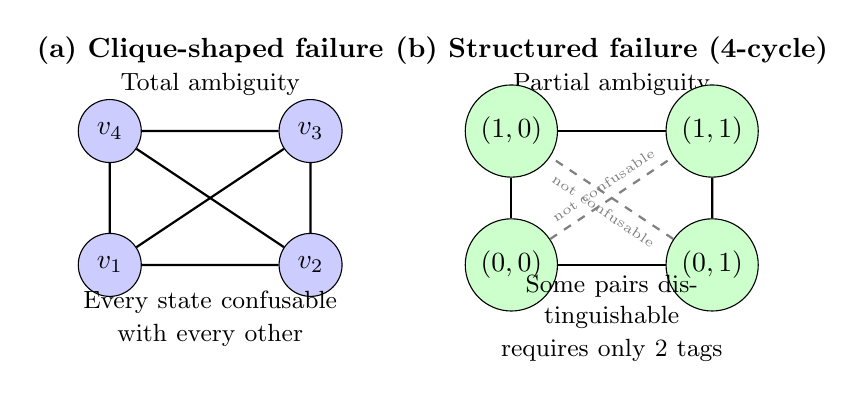
\begin{tikzpicture}[scale=0.85]
  % Panel A: Clique
  \begin{scope}[xshift=0cm]
    \node at (1.5, 3.2) {\textbf{(a) Clique-shaped failure}};
    \node at (1.5, 2.7) {\small Total ambiguity};
    
    % Four vertices in a square
    \node[circle, draw, fill=blue!20, minimum size=8mm] (a1) at (0, 0) {$v_1$};
    \node[circle, draw, fill=blue!20, minimum size=8mm] (a2) at (3, 0) {$v_2$};
    \node[circle, draw, fill=blue!20, minimum size=8mm] (a3) at (3, 2) {$v_3$};
    \node[circle, draw, fill=blue!20, minimum size=8mm] (a4) at (0, 2) {$v_4$};
    
    % All edges (clique)
    \draw[thick] (a1) -- (a2) -- (a3) -- (a4) -- (a1);
    \draw[thick] (a1) -- (a3);
    \draw[thick] (a2) -- (a4);
    
    \node[text width=3.5cm, align=center] at (1.5, -0.8) {\small Every state confusable\\with every other};
  \end{scope}
  
  % Panel B: 4-cycle
  \begin{scope}[xshift=6cm]
    \node at (1.5, 3.2) {\textbf{(b) Structured failure (4-cycle)}};
    \node at (1.5, 2.7) {\small Partial ambiguity};
    
    % Four vertices in a square
    \node[circle, draw, fill=green!20, minimum size=8mm] (b1) at (0, 0) {$(0,0)$};
    \node[circle, draw, fill=green!20, minimum size=8mm] (b2) at (3, 0) {$(0,1)$};
    \node[circle, draw, fill=green!20, minimum size=8mm] (b3) at (3, 2) {$(1,1)$};
    \node[circle, draw, fill=green!20, minimum size=8mm] (b4) at (0, 2) {$(1,0)$};
    
    % Cycle edges only
    \draw[thick] (b1) -- (b2);
    \draw[thick] (b2) -- (b3);
    \draw[thick] (b3) -- (b4);
    \draw[thick] (b4) -- (b1);
    
    % Dashed lines for non-edges
    \draw[dashed, gray, thick] (b1) -- (b3) node[midway, above, sloped, font=\tiny] {not confusable};
    \draw[dashed, gray, thick] (b2) -- (b4) node[midway, below, sloped, font=\tiny] {not confusable};
    
    \node[text width=3.5cm, align=center] at (1.5, -0.8) {\small Some pairs distinguishable\\requires only 2 tags};
  \end{scope}
\end{tikzpicture}
\caption{Two failure topologies. In (a), the observation provides no discrimination, so the confusability graph is a clique: every state is confusable with every other, and exact recovery requires a tag for each state. In (b), partial observations provide some discrimination: opposite corners are distinguishable even though adjacent states are not. The 4-cycle is 2-colorable, so exact recovery requires only 2 tags. This structural difference is invisible to the unit-rate threshold alone.}
\label{fig:failure-topology}
\end{figure}
